% Supporting Information — standalone supplement for
% "Measurement Inheritance: Following a Doxy-PEP Bystander-Resistance Signal from
%  Trial to Surveillance"  (Demidont). Compiles independently of the main manuscript.
%
% Figures: \graphicspath points at ../outputs/figures for in-repo compilation, while
% \includegraphics uses bare filenames so the same file compiles in a flat submission
% folder (drop the three PNGs next to this .tex and the graphicspath line is harmless).
%   pdflatex supplementary.tex
\documentclass[11pt]{article}
\usepackage[T1]{fontenc}
\usepackage[utf8]{inputenc}
\usepackage{lmodern}
\usepackage{amsmath,amssymb}
\usepackage{textcomp}
\usepackage{graphicx}
\usepackage[margin=1in]{geometry}
\usepackage[hidelinks]{hyperref}
\usepackage{url}\urlstyle{tt}
\usepackage{parskip}
\usepackage{caption}
\captionsetup{labelformat=empty,justification=raggedright,singlelinecheck=false,font=small}
\graphicspath{{../outputs/figures/}{.}}

\newcommand{\Sa}{\textit{S.~aureus}}

\title{\textbf{Supporting Information}\\[6pt]
\large Measurement Inheritance: Following a Doxy-PEP Bystander-Resistance
Signal from Trial to Surveillance}
\author{Adrian C. Demidont, DO}
\date{}

\begin{document}
\maketitle
\thispagestyle{empty}

All supplementary material regenerates from the public repository (\texttt{make all};
\texttt{outputs/}) and is deposited with the archive.

\section*{S1 Text. Supplementary Stream A analyses and Stream C dilution analyses}

\subsection*{Stream A supplementary analyses}

The deeper trial-reanalyses that establish the cross-sectional carriage endpoint could
not resolve the downstream population question under the observed designs and sampling
structure, and are not load-bearing for
the individual-level result: the DoxyPEP and DOXYVAC carriage trajectories (non-monotone,
arm-crossing); the between-cohort MRSA-colonisation dispersion used as an external
heterogeneity anchor (\path{outputs/dejong_sigma_result.md}); the resulting inflation
of a naive cross-sectional trend test (\path{outputs/coverage_null_result.md}); the
non-identifiability of outbreak shape (\path{outputs/three_outbreak_fit_result.md});
the interim power and duration multiples (\path{outputs/detectability_result.md},
\path{outputs/duration_result.md}); and a cross-organism example of mechanism-blind
measurement (a military antimalarial--doxycycline cohort in which overall resistance did
not differ by exposure while \textit{tet}(M) genes did).

\subsection*{Stream C dilution leg (Figures A--C)}

Even a linked surveillance system would face an exposed subgroup too dilute to move a
population rate under the realistic configurations evaluated.

\begin{figure}[h]
\centering
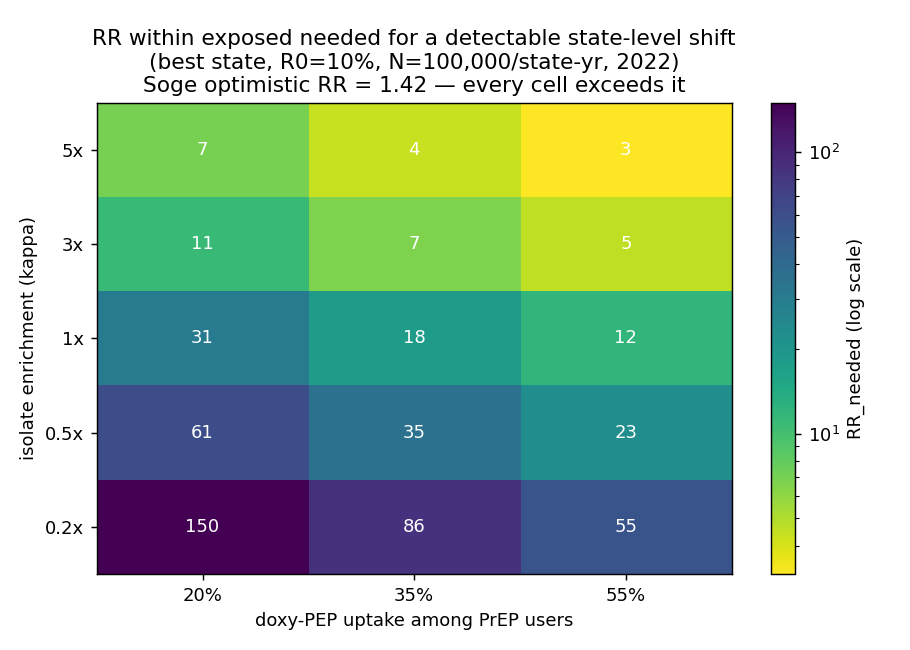
\includegraphics[width=0.82\textwidth,keepaspectratio]{feasibility_dilution.png}
\caption{Figure A. State level. Within-exposed relative risk required for a detectable
state-level shift in tetracycline non-susceptibility, over doxy-PEP uptake $\times$ isolate
enrichment (best state, $R_0 = 10\%$, $N = 100\,000$/state-year). Every cell exceeds Soge's
optimistic $\mathrm{RR} = 1.42$.}
\end{figure}

\begin{figure}[h]
\centering
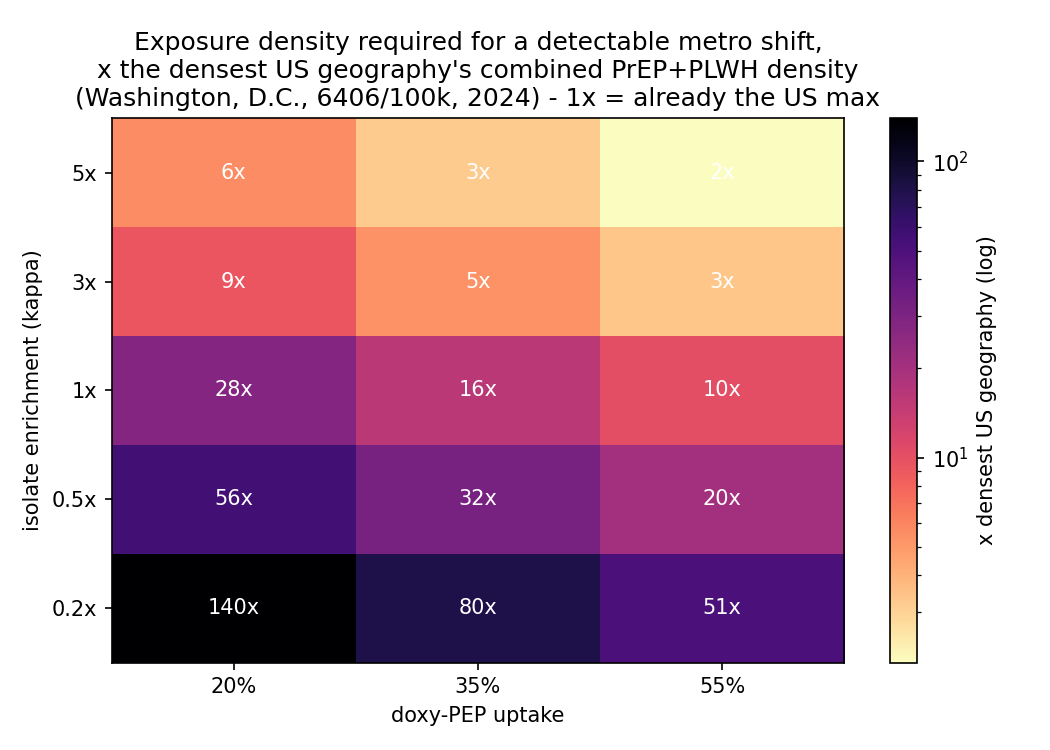
\includegraphics[width=0.82\textwidth,keepaspectratio]{feasibility_metro.png}
\caption{Figure B. Metro level. Male-PrEP density required for a detectable shift, as
multiples of the densest US geography (Washington, D.C.). $1\times$ is already the national
maximum.}
\end{figure}

\begin{figure}[h]
\centering
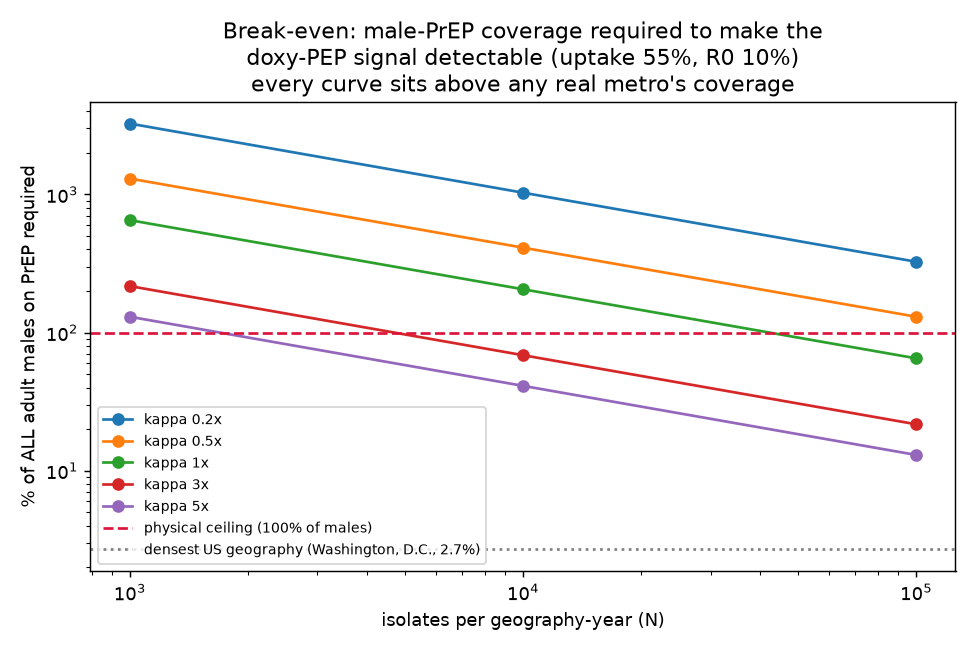
\includegraphics[width=0.82\textwidth,keepaspectratio]{feasibility_metro_breakeven.png}
\caption{Figure C. Break-even in proxy-free units. Share of \emph{all} adult males on
PrEP required for detection versus isolates per geography-year, by enrichment $\kappa$.
Every curve sits above D.C.'s observed 2.7\% and, under realistic isolate volumes, above
the 100\%-of-males physical ceiling.}
\end{figure}

\end{document}
